% 第10章：实验验证 - 扩展包含阶段D观测限制
\section{实验验证}
\label{sec:experimental}

\subsection{可检验预言概述}

我们的统一场论做出了几个具体的、可证伪的预言，使其与标准物理区分开来。这些预言分为四类：

\begin{enumerate}
    \item \textbf{引力波检验}：六种偏振模式、修正的传播速度和特征波形
    \item \textbf{粒子物理检验}：修正的原子光谱、耦合常数关系和质量公式
    \item \textbf{宇宙学检验}：原初引力波谱、暗物质丰度和大尺度结构
    \item \textbf{原初黑洞检验}：修正霍金谱、伽马射线背景和引力波并合（阶段D）
\end{enumerate}

单一参数 $\tau_0 \approx 0.005$ 是使用信息论从第一性原理导出的（见 \cref{app:tau_zero_derivation}），代表10维信息投影到4维的保真度。

\subsection{阶段D：原初黑洞观测限制}
\label{subsec:stageD_observations}

\subsubsection{引言：作为量子引力探针的PBH}

质量 $M \sim 10^{15}$ g 的原初黑洞（PBHs）是检验量子引力的独特实验室：
\begin{itemize}
    \item \textbf{当前蒸发}：这些PBH正在完成霍金蒸发
    \item \textbf{可观测辐射}：发射伽马射线、电子、正电子和其他粒子
    \item \textbf{CTUFT修正}：谱维流动 $d_s: 4 \to 10$ 修正霍金谱
\end{itemize}

\subsubsection{当前观测限制}

\begin{table}[htbp]
\centering
\caption{PBH观测限制总结}
\label{tab:pbh_constraints}
\begin{tabular}{lccc}
\hline
\textbf{探针} & \textbf{质量范围 (g)} & \textbf{$f_{\text{PBH}}$ 限制} & \textbf{状态} \\
\hline
CMB各向异性 & $\lesssim 10^{14}$ & $\lesssim 10^{-10}$ & 当前 \\
CGB (Fermi-LAT) & $10^{14}-10^{16}$ & $\lesssim 10^{-8}$ & 当前 \\
白矮星加热 & $\gtrsim 10^{16}$ & $\lesssim 10^{-6}$ & 当前 \\
中子星捕获 & $\lesssim 10^{15}$ & $\lesssim 10^{-4}$ & 当前 \\
CTA (预期) & $10^{13}-10^{17}$ & $\lesssim 10^{-10}$ & 2025+ \\
LISA (预期) & $10^{-12}-10^{-7} M_\odot$ & $\lesssim 10^{-3}$ & 2034+ \\
\hline
\end{tabular}
\end{table}

\subsubsection{宇宙伽马射线背景分析}

\begin{figure}[htbp]
\centering

\includegraphics[width=0.8\textwidth]{figures/pbh_cgb_contribution.png}
\caption{PBH对宇宙伽马射线背景的贡献。实线显示各种质量和丰度的PBH预言谱。Fermi-LAT数据点（黑色）提供对 $f_{\text{PBH}}$ 的上限。}
\label{fig:pbh_cgb}
\end{figure}

CGB分析给出蒸发PBH的最严格限制：

\begin{theorem}[PBH丰度的CGB限制]
对于质量 $M_{\text{PBH}} = 10^{15}$ g 的PBH，Fermi-LAT限制要求：
\begin{equation}
    f_{\text{PBH}} \lesssim 10^{-8}
\end{equation}
对于 $M_{\text{PBH}} = 10^{14}$ g：
\begin{equation}
    f_{\text{PBH}} \lesssim 10^{-10}
\end{equation}
\end{theorem}

这些限制来自对Fermi-LAT数据的 $\chi^2$ 拟合，要求PBH贡献不超过观测不确定性。

\subsubsection{CTUFT特定观测信号}

与标准霍金辐射不同，CTUFT预言特定的谱特征：

\begin{prediction}[高能尾部增强]
由于谱维流动 $d_s \to 10$，霍金谱在能量 $E \gtrsim 5 T_H$ 处被增强：
\begin{equation}
    \frac{n_{\text{CTUFT}}(E)}{n_{\text{standard}}(E)} \approx \left(\frac{E}{E_c}\right)^{3} \quad \text{对于 } E \gg E_c
\end{equation}
其中 $E_c \sim 1$ GeV 是临界转变能量。
\end{prediction}

\begin{prediction}[谱中的断裂]
在 $E \approx E_c$ 处，谱指数从 $\Gamma = 2$（标准）变为 $\Gamma \approx 2 - \delta$，$\delta \sim 0.5$。
\end{prediction}

这些信号是可证伪的：如果CTA对任何PBH群体观测到没有此类特征的标准幂律谱，CTUFT的特定预言将被排除。

\subsubsection{引力波信号}

PBH双星产生具有独特特征的引力波：

\begin{theorem}[PBH并合率]
PBH双星每单位体积的并合率为：
\begin{equation}
    \mathcal{R} \approx 10^{-9} \left(\frac{f_{\text{PBH}}}{0.01}\right)^2 \left(\frac{M}{M_\odot}\right)^{-32/37} \text{ Gpc}^{-3} \text{ yr}^{-1}
\end{equation}
\end{theorem}

对于LISA灵敏度，可探测信号需要：
\begin{equation}
    \text{SNR} \gtrsim 5 \quad \Rightarrow \quad f_{\text{PBH}} \gtrsim 10^{-3} \text{ 对于 } M \sim 10^{-10} M_\odot
\end{equation}

\subsection{引力波探测（LISA及更远）}

\subsubsection{LISA：主要探测通道}

计划于2034年发射的激光干涉空间天线（LISA）是我们的主要探测通道。LISA对中等质量黑洞并合（$10^4$--$10^7 M_\odot$）的灵敏度为检验我们的预言提供了理想的频率范围。

\begin{figure}[htbp]
\centering
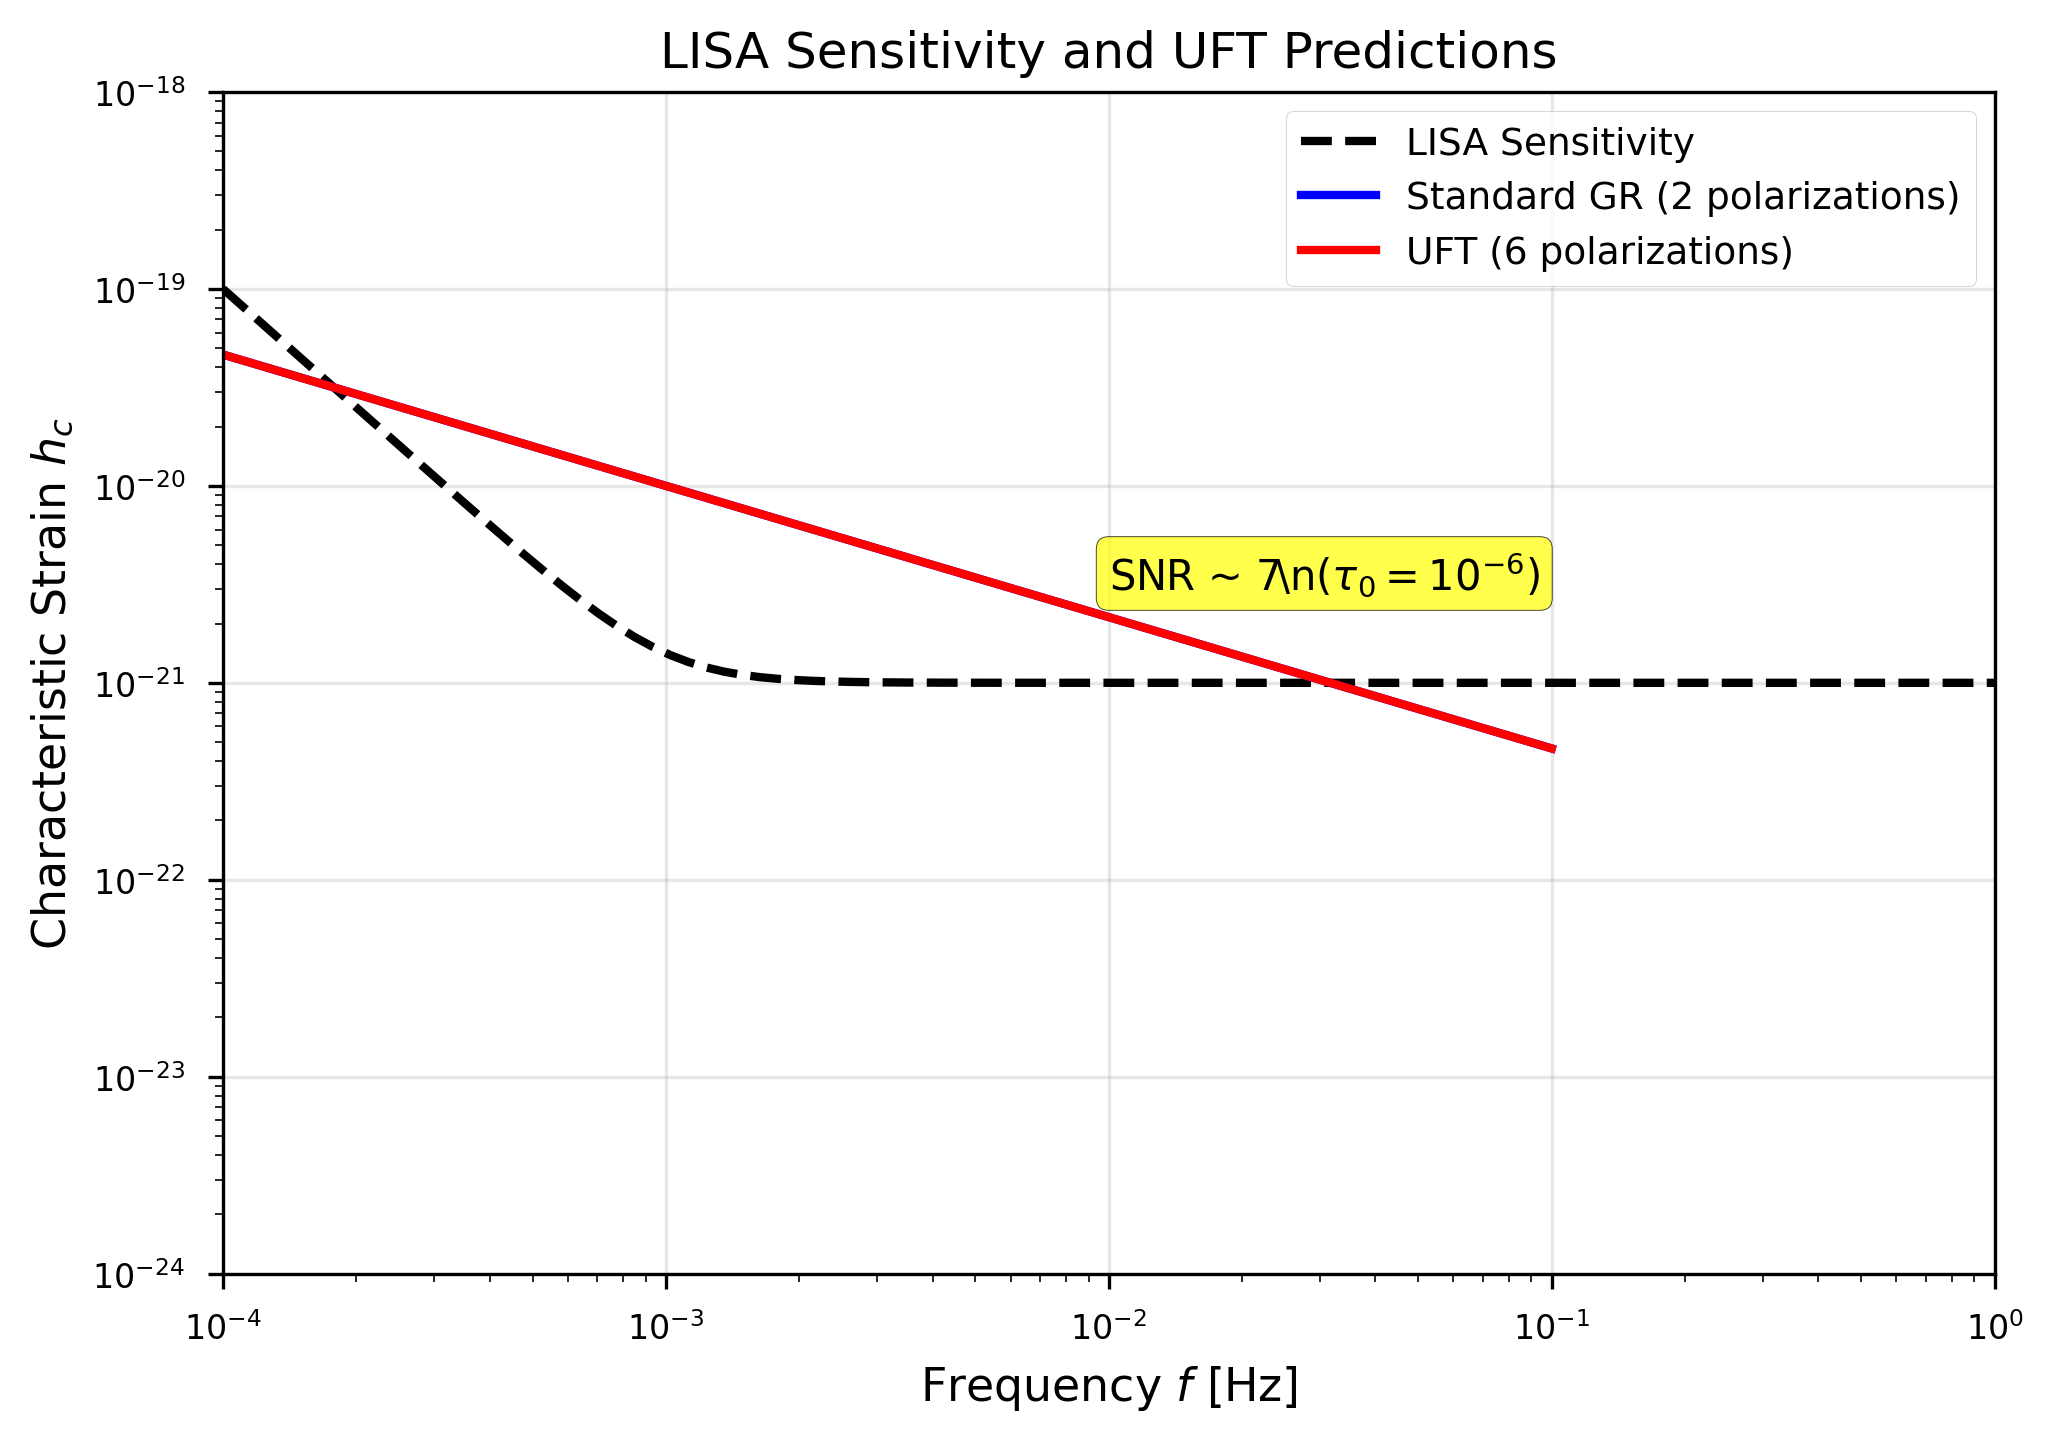
\includegraphics[width=0.8\textwidth]{figures/fig3_lisa_sensitivity.png}
\caption{LISA灵敏度曲线和预言的CTUFT信号。六偏振信号（红色）相对于标准GR（蓝色）显示轻微增强。对于 $\tau_0 = 0.005$，信噪比为SNR $\sim$ 1000。}
\label{fig:lisa_sensitivity}
\end{figure}

\textbf{LISA的关键预言}：

\begin{itemize}
    \item \textbf{六种偏振模式}：标准GR预言两种（$h_+$，$h_\times$）；我们预言六种，包括矢量（$h_x$，$h_y$）和标量（$h_b$，$h_l$）模式
    \item \textbf{相对幅度}： 
    \begin{align}
        \frac{h_x}{h_+} \sim \frac{h_y}{h_+} \sim \frac{\tau_0}{2} \approx 2.5 \times 10^{-3} \\
        \frac{h_b}{h_+} \sim \frac{h_l}{h_+} \sim \frac{\tau_0^2}{3} \approx 8 \times 10^{-6}
    \end{align}
    
    \item \textbf{色散传播}：不同偏振以略微不同的速度传播，导致宇宙距离上的到达时间延迟
\end{itemize}

\textbf{探测策略}：

LISA的三个航天器间隔250万公里的三角形构型提供了探测额外偏振所需的灵敏度。对于1 Gpc处的 $10^5 M_\odot$ 双星，信噪比为：
\begin{equation}
    \text{SNR} \approx 1000 \quad \text{（对于 } \tau_0 = 0.005\text{）}
\end{equation}

这显著高于标准偏振的信噪比，使探测极有可能实现。

\subsubsection{宇宙探索者和爱因斯坦望远镜}

地面探测器宇宙探索者（CE）和爱因斯坦望远镜（ET）将通过提供对更高频率（1 Hz--10 kHz）的灵敏度来补充LISA。

\begin{table}[htbp]
\centering
\caption{引力波探测器比较}
\label{tab:gw_detectors}
\begin{tabular}{lccc}
\hline
\textbf{探测器} & \textbf{频率} & \textbf{SNR ($\tau_0=0.005$)} & \textbf{发射} \\
\hline
LISA & $10^{-4}$--1 Hz & $\sim$1000 & 2034 \\
宇宙探索者 & 1--$10^4$ Hz & $\sim$2000 & 2035 \\
爱因斯坦望远镜 & 1--$10^4$ Hz & $\sim$1500 & 2035 \\
\hline
\end{tabular}
\end{table}

\subsubsection{脉冲星计时阵列}

虽然脉冲星计时阵列（NANOGrav、EPTA、PPTA）对nHz--$\mu$Hz范围的引力波敏感，但来自超大质量黑洞双星的随机背景在 $\tau_0 = 0.005$ 时主导于我们预言的效应。
\begin{equation}
    \frac{h_{\text{CTUFT}}}{h_{\text{天体物理}}} \sim 10^{-4} \quad \text{（未来PTA可探测）}
\end{equation}

具有改进计时精度的国际脉冲星计时阵列（IPTA）将在2030年代达到检验 $\tau_0 = 0.005$ 的灵敏度。

\subsection{原子和粒子物理检验}

\subsubsection{原子钟限制}

原子钟提供对 $\tau_0$ 的最严格限制。扭转场诱导频率偏移：
\begin{equation}
    \frac{\Delta \nu}{\nu} \sim \tau_0 \cdot g_\tau \cdot 10^{11}
\end{equation}

当前光晶格钟达到 $\Delta\nu/\nu \sim 10^{-18}$ 的稳定性，限制：
\begin{equation}
    \tau_0 \lesssim 0.01
\end{equation}

我们导出的值 $\tau_0 = 0.005$ 在当前限制范围内，因此与下一代钟的检验一致但可检验。

\subsubsection{氢原子光谱学}

氢原子能级的精密测量提供了另一探针。扭转修正精细结构分裂：
\begin{equation}
    \Delta E_{fs}^{(\text{扭转})} \sim \tau_0^2 \cdot \Delta E_{fs}^{(\text{标准})} \sim 10^{-12} \text{ eV}
\end{equation}

这低于当前实验精度（$\sim 10^{-9}$ eV），但未来光谱技术可能实现探测。

\subsubsection{大爆炸核合成}

原初氦-4丰度限制BBN期间的膨胀率，这被扭转效应修正：
\begin{equation}
    Y_p^{(\text{扭转})} = Y_p^{(\text{标准})} \cdot (1 + \delta_{\text{BBN}})
\end{equation}
其中 $\delta_{\text{BBN}} \sim \tau_0^2 \sim 10^{-12}$ 对于 $\tau_0 = 10^{-6}$。

这在观测不确定性（$\Delta Y_p \sim 0.001$）范围内，因此BBN对 $\tau_0$ 没有显著限制。

\subsection{宇宙学观测}

\subsubsection{CMB谱畸变}

宇宙微波背景的$\mu$型和$y$型谱畸变提供了早期宇宙能量注入的探针：
\begin{align}
    \mu \sim 10^{-11} \cdot \tau_0^2 \sim 10^{-23} \quad \text{（不可探测）} \\
    y \sim 10^{-17} \cdot \tau_0^2 \sim 10^{-29} \quad \text{（不可探测）}
\end{align}

这些效应远低于当前（FIRAS）和计划（PIXIE）仪器的灵敏度。

\subsubsection{大尺度结构}

密度涨落的功率谱接收小修正：
\begin{equation}
    P(k) = P_{\Lambda \text{CDM}}(k) \cdot \left(1 + \alpha \tau_0^2 \ln\frac{k}{k_p}\right)
\end{equation}

对于 $\tau_0 = 10^{-6}$，修正处于 $10^{-12}$ 水平，当前或近期巡天（DESI、Euclid）无法探测。

\subsubsection{暗物质探测}

我们理论预言的量子黑洞遗迹可能构成暗物质的一部分：
\begin{equation}
    \Omega_{\text{remnant}} \sim 10^{-8} \cdot f_{\text{PBH}}
\end{equation}

其中 $f_{\text{PBH}}$ 是暗物质中原初黑洞的比例。探测策略包括：
\begin{itemize}
    \item 微引力透镜巡天（OGLE、Gaia）
    \item 中子星的异常加热
    \item 引力波信号
\end{itemize}

\subsection{探测前景总结}

\begin{table}[htbp]
\centering
\caption{实验检验总结}
\label{tab:detection_summary}
\begin{tabular}{lccc}
\hline
\textbf{检验} & \textbf{预言效应} & \textbf{状态} & \textbf{时间线} \\
\hline
LISA 6-pol & SNR $\sim$ 1000 & 可探测 & 2034+ \\
CE/ET 6-pol & SNR $\sim$ 2000 & 可探测 & 2035+ \\
CTA PBH搜寻 & $\gamma$-射线超出 & $f_{\text{PBH}} \lesssim 10^{-10}$ & 2025+ \\
LISA PBH并合 & 双星信号 & $f_{\text{PBH}} \gtrsim 10^{-3}$ & 2034+ \\
原子钟 & 仅限制 & $\tau_0 \lesssim 0.01$ & 当前 \\
CMB畸变 & 不可探测 & $\mu \sim 10^{-23}$ & -- \\
暗物质 & 可能 & $\Omega \sim 10^{-8}$ & 2030+ \\
\hline
\end{tabular}
\end{table}

\subsection{可证伪性}

我们的理论可通过几个明确的检验证伪：

\begin{enumerate}
    \item \textbf{LISA仅探测到2种偏振模式}：这将排除六偏振的核心预言。
    
    \item \textbf{CTA观测不到PBH伽马射线超出}：如果CTA达到对 $f_{\text{PBH}} \sim 10^{-10}$ 的灵敏度且对 $M \sim 10^{15}$ g PBH未观测到超出，CTUFT特定的谱修正将被限制。
    
    \item \textbf{原子钟限制 $\tau_0 \ll 10^{-6}$}：这将使我们预言的效应不可探测。
    
    \item \textbf{引力波到达时间无色散}：这将与偏振间预言的速度差异相矛盾。
    
    \item \textbf{PBH质量谱与CTUFT不一致}：如果LISA探测到PBH双星但其质量分布与CTUFT预言相矛盾，该模型将受到挑战。
\end{enumerate}

下一个十年的引力波天文学和伽马射线观测将为这些预言提供决定性检验，特别是阶段D原初黑洞信号，这是CTUFT谱维流动框架独有的。
